\section{Prototyping}

In this project a very big part has been prototyping and sketching. 

The most important part of the overall design happened in the sketching phase, all most all activities and their screens was made in this periode. 

Prototyping was also important in this project because before the programmingstarted out, a prototype was represented to the \guardian{}s from \egebakken{}. This was a papir-prototype and showed both how the screens was ment to be implemented and designed and how the flow in the program was going to be. This was done so the \guardian{}s could come with feedback on which screens or activities should be changed as it was important to hear what the costumer had to say. An overview of this prototype can be seen in \autoref{fig:first_prototype}

\begin{figure}[h!]
	\centering
	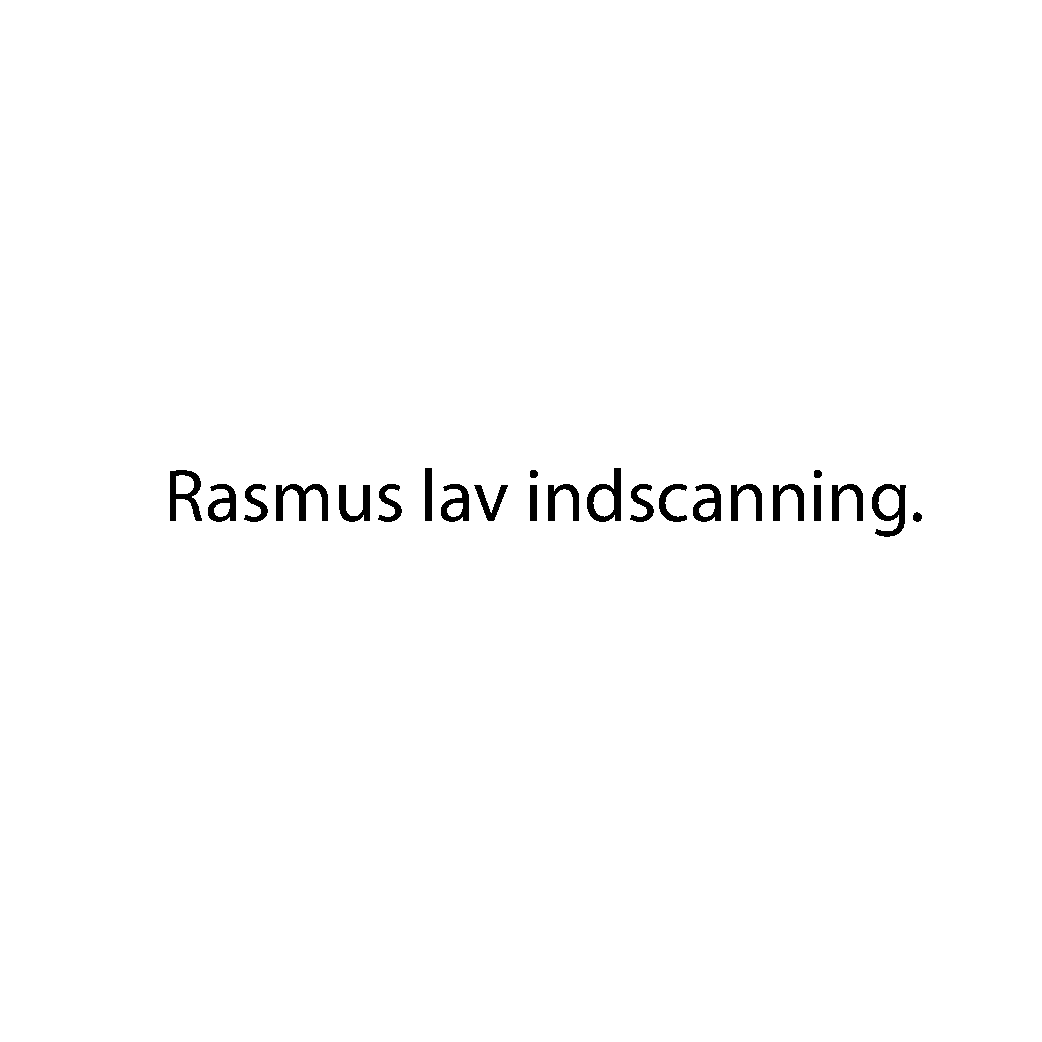
\includegraphics[width=1\textwidth]{gfx/first-prototype.pdf}
	\caption{Overview from the first Prototype.}
	\label{fig:first_prototype}
\end{figure}
